\documentclass[12pt,oneside,a4paper]{scrartcl}

\usepackage[left=2cm,right=1.5cm,top=1cm,bottom=1cm,includeheadfoot]{geometry}
\usepackage[T1]{fontenc}
%\usepackage[scaled]{helvet}
%\usepackage{times}
%\usepackage[scaled]{beramono}
\newcommand{\mono}[1]{\texttt{\footnotesize{#1}}}

\usepackage[utf8]{inputenc}
\usepackage[ngerman]{babel}

% header & footer
\usepackage{fancyhdr}
\pagestyle{fancy}
\fancyhf{}
\fancyhead[L]{\nouppercase{\small 185.A01 OOP Übung 2 - Spezifikation}}
\fancyhead[R]{\nouppercase{\small \today}}
\renewcommand{\headrulewidth}{0.5pt}
\fancyfoot[L]{\small Gruppe 169}
\fancyfoot[R]{\small \thepage}
\renewcommand{\footrulewidth}{0.5pt}

% Math stuff
\usepackage{amsmath}
\usepackage{amssymb}
\usepackage{mathtools}
\usepackage{multirow}

% font colors
\usepackage{color}
\definecolor{orange}{RGB}{255,127,0}
\definecolor{green}{RGB}{0,127,0}
\definecolor{lblue}{RGB}{63,63,255,0}
% used in ListingBox
\definecolor{red}{RGB}{255,0,0}
\definecolor{lgrey}{RGB}{223,223,223,0}
\definecolor{brown}{RGB}{0.5,0.5,0.25}
\definecolor{blue}{RGB}{0,0,255}
\definecolor{purple}{rgb}{0.7,0,0.7}

\usepackage{graphicx}
\usepackage{tabularx}
\usepackage{hyperref}
\usepackage{hyperref}
\hypersetup
{
	colorlinks,
	citecolor=black,
	filecolor=black,
	linkcolor=black,
	urlcolor=black
}

\include{CodeListingBox}


\begin{document}

\begin{titlepage}

\begin{center}
%\vspace*{0.5cm}
%\begin{figure}[htbp]
%	\centering
%	\includegraphics[scale=1]{figures/INF_Logo_typo_grau}
%\end{figure}
\vspace*{1cm}
\sffamily \Large Übung 2\\[0.7cm]
\rule{\linewidth}{1pt} \\[0.3cm]
\LARGE 185.A01 Objektorientierte Programmiertechniken \\
\rule{\linewidth}{1pt} \\[1cm]

\normalfont \Large Goran Filcic \\[0.3cm]
\normalsize Matr. Nr.: 1025112 \\[0.1cm]
e1025112@student.tuwien.ac.at \\[0.8cm]

\normalfont \Large Manuel Schmitt\\[0.3cm]
\normalsize Matr. Nr.: 1127688 \\[0.1cm]
e1127688@student.tuwien.ac.at \\[0.8cm]


\normalfont \Large Peter Nirschl \\[0.3cm]
\normalsize Matr. Nr.: 1025647 \\[0.1cm]
e1025647@student.tuwien.ac.at \\[0.8cm]



\Large \today \normalfont
\end{center}
\end{titlepage}

\setcounter{page}{1}
\tableofcontents

\newpage

\section{Einleitung}
Die bestehende Codebase wird von der Gruppe erweitert, sodass es möglich sein wird mit dem Programm effektiv zu arbeiten.

\section{Analyse der Anwendungsfälle}
\begin{center}
	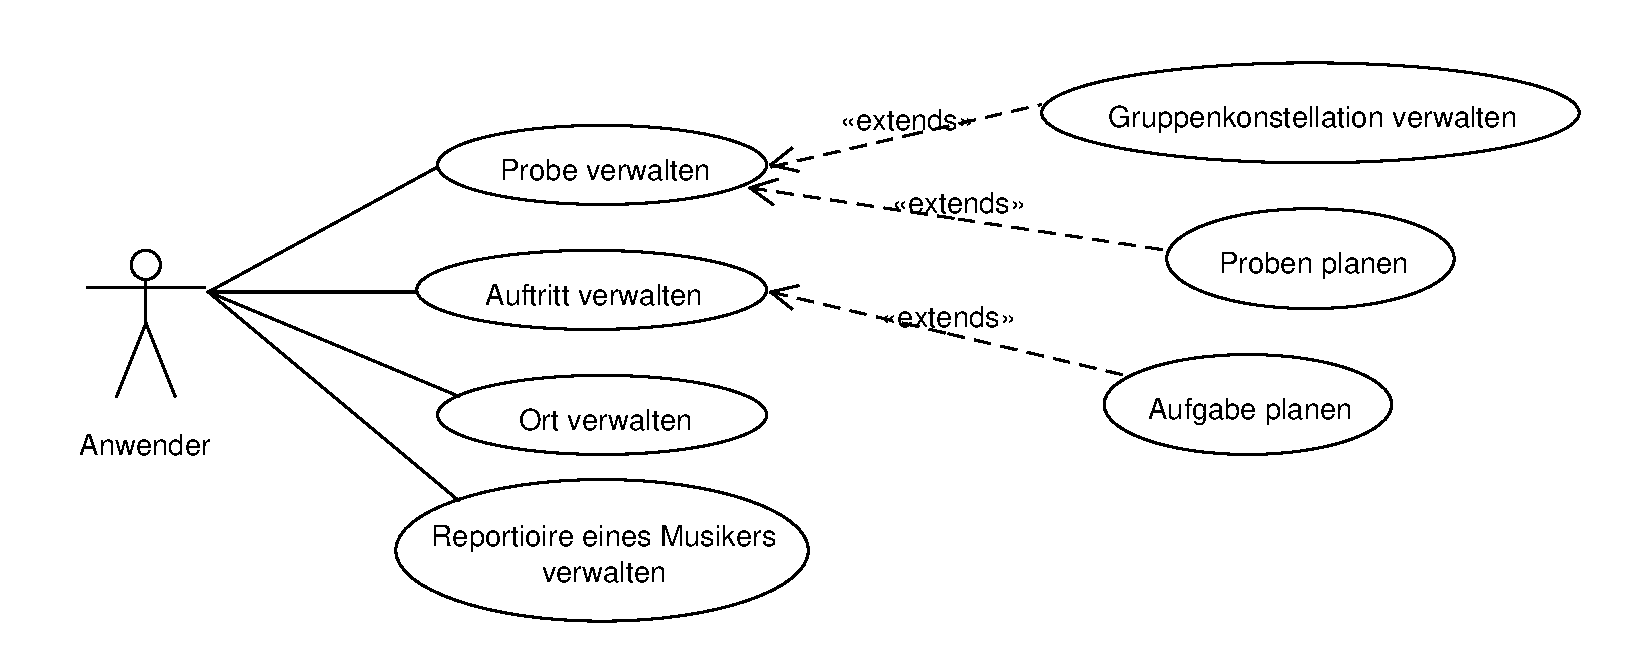
\includegraphics[width=1\textwidth]{usecase.pdf}
\end{center}


\section{Beschreibung der Anforderungen}
\subsection{Annahmen und Voraussetzungen}
\begin{enumerate}
	\item Das System unterscheidet (noch) nicht zwischen verschiedenen Benutzergruppen.
	\item Das System wird zu einem Zeitpunkt von genau einem Benutzer verwendet.
	% Bitte ergänzen falls euch noch etwas einfällt
\end{enumerate}

\subsection{Allgemeine Beschreibung}
Folgende Funktionalitäten sind zu implementieren (eine genauere Beschreibung erfolgt weiter unten):
\begin{enumerate}
	\item Persistenz der Daten
	\item Unterscheidung zwischen vergangenen (bestätigten) Ereignissen und zukünftigen Ereignissen
	\item Verwaltung von Proben und Auftritten (inklusive Historisierung der Daten)
	\item Verwaltung von Orten
\end{enumerate}

\subsection{Detailierte Beschreibung}
\subsubsection*{Persistenz der Daten}
Der Zustand der Entitäten soll nach der Manipulation des Datenbestandes persisitiert werden.
Dazu wird die Klasse \texttt{Musikgruppe} dahingehend erweitert, dass sie alle Unterobjekte
in einer XML-Struktur abspeichert. Die Unterobjekte müssen ebenfalls erweitert werden.
Damit die Objekte alle gleich strukturiert sind, wird ein Interface \texttt{IPersistent} eingeführt:

\begin{figure}[htbp]
	\centering
	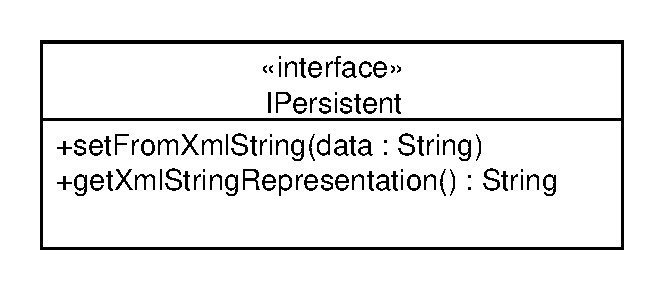
\includegraphics[width=5.0cm]{ipersistent.pdf}
	\caption{Definition der IPersistent Schnittstelle}
	\label{image:ipersistent}
\end{figure}



\subsubsection*{Vergangenheit und Zukunft}
Die Entität \texttt{Ereignis} wird so erweitert, dass eindeutig feststellbar ist ob das Ereignis bestätigt ist oder nicht.
Bestätigte Ereignisse werden aus Performance-Gründen getrennt von zukünftigen (planbaren) Ereignissen im Speicher gehalten.


\subsubsection*{Verwaltung von Proben und Auftritten}
Proben und Auftritte können verändert und entfernt werden. Veränderungen müssen nachvollziehbar im System abgebildet sein.

Pro Probe (bzw. Auftritt) kann eine eigene Konstellation an Musikern angegeben werden.
Die Musiker werden aufgeteilt in permanente Mitglieder und Ersatzmitglieder.


\subsubsection*{Verwaltung von Orten}
Orte werden als zusätzliche Entität im System abgebildet und können von Benutzern verwaltet werden.
Zur Nachvollziehbarkeit werden Orte nicht gelöscht. Alle Änderungen an Orten müssen nachvollziehbar sein.


\section{Details zur Umsetzung}
\subsection{Verteilung der Verantwortung}
Die Verantwortung zur Umsetzung 
 
\begin{figure}[h!]
%\begin{table}
    \begin{tabular}{l|l}
        Mitglied       & Arbeitspakete \\ \hline \hline
        Goran Filcic   & Trennung vergangener u. zukünftiger Ereignisse \\ 
        Manuel Schmitt & Verwaltung von Reportoire, Orten und Gruppenkonstellationen\\ 
        Peter Nirschl  & Persistenz d. Daten \\
    \end{tabular}
%\end{table}
\end{figure}

\end{document}
